\documentclass[a4paper, toc=index,abstract=true]{scrartcl}\usepackage[]{graphicx}\usepackage[]{color}
%% maxwidth is the original width if it is less than linewidth
%% otherwise use linewidth (to make sure the graphics do not exceed the margin)
\makeatletter
\def\maxwidth{ %
  \ifdim\Gin@nat@width>\linewidth
    \linewidth
  \else
    \Gin@nat@width
  \fi
}
\makeatother

\definecolor{fgcolor}{rgb}{0.345, 0.345, 0.345}
\newcommand{\hlnum}[1]{\textcolor[rgb]{0.686,0.059,0.569}{#1}}%
\newcommand{\hlstr}[1]{\textcolor[rgb]{0.192,0.494,0.8}{#1}}%
\newcommand{\hlcom}[1]{\textcolor[rgb]{0.678,0.584,0.686}{\textit{#1}}}%
\newcommand{\hlopt}[1]{\textcolor[rgb]{0,0,0}{#1}}%
\newcommand{\hlstd}[1]{\textcolor[rgb]{0.345,0.345,0.345}{#1}}%
\newcommand{\hlkwa}[1]{\textcolor[rgb]{0.161,0.373,0.58}{\textbf{#1}}}%
\newcommand{\hlkwb}[1]{\textcolor[rgb]{0.69,0.353,0.396}{#1}}%
\newcommand{\hlkwc}[1]{\textcolor[rgb]{0.333,0.667,0.333}{#1}}%
\newcommand{\hlkwd}[1]{\textcolor[rgb]{0.737,0.353,0.396}{\textbf{#1}}}%
\let\hlipl\hlkwb

\usepackage{framed}
\makeatletter
\newenvironment{kframe}{%
 \def\at@end@of@kframe{}%
 \ifinner\ifhmode%
  \def\at@end@of@kframe{\end{minipage}}%
  \begin{minipage}{\columnwidth}%
 \fi\fi%
 \def\FrameCommand##1{\hskip\@totalleftmargin \hskip-\fboxsep
 \colorbox{shadecolor}{##1}\hskip-\fboxsep
     % There is no \\@totalrightmargin, so:
     \hskip-\linewidth \hskip-\@totalleftmargin \hskip\columnwidth}%
 \MakeFramed {\advance\hsize-\width
   \@totalleftmargin\z@ \linewidth\hsize
   \@setminipage}}%
 {\par\unskip\endMakeFramed%
 \at@end@of@kframe}
\makeatother

\definecolor{shadecolor}{rgb}{.97, .97, .97}
\definecolor{messagecolor}{rgb}{0, 0, 0}
\definecolor{warningcolor}{rgb}{1, 0, 1}
\definecolor{errorcolor}{rgb}{1, 0, 0}
\newenvironment{knitrout}{}{} % an empty environment to be redefined in TeX

\usepackage{alltt}
\usepackage{gensymb}
\usepackage{geometry}
\usepackage{enumitem}
\usepackage{setspace}
\usepackage{booktabs}
\usepackage{subfig}
\usepackage{placeins}
\usepackage{amsmath}
\usepackage{pdflscape}
\usepackage{multirow}
\usepackage{longtable}
\usepackage[toc,page]{appendix}
\usepackage{array,booktabs}
\usepackage[american]{babel}
\usepackage[backend=biber,
mincitenames = 1,
maxcitenames = 1,
uniquename = false,
uniquelist = false,
citestyle = authoryear-comp]{biblatex}%
\usepackage{lineno, blindtext}
\addbibresource{Sizing-fx-of-temperature.bib}
\captionsetup[table]{singlelinecheck=false}

\title{Beyond conceptual eco-physiological hypotheses: insights from a general size and trait-based model of ectotherm thermal performance}
\author{Philipp Neubauer\\Dragonfly Data Science, Wellington, NZ  \and 
        Ken H. Andersen\\Centre for Ocean Life
        Danish Technical University, Lyngby, Denmark}
\IfFileExists{upquote.sty}{\usepackage{upquote}}{}
\begin{document}

\maketitle

\begin{spacing}{1.9}

\pagenumbering{gobble}
\begin{abstract}

Increasing temperatures under climate change are thought to affect individual physiology of ectotherms through increases in metabolic demands, leading to changes in species performance with concomitant effects on species ecology. Although intuitively appealing, the driving mechanisms behind thermal performance is contested: thermal performance (e.g., growth) appears correlated with metabolic scope (i.e., oxygen availability for activity) for a number of species, but a substantial number of datasets do not support oxygen limitation of long-term performance. Whether or not oxygen limitations via the metabolic scope, or a lack thereof, have major ecological consequences remains a highly contested question. Here, we propose a general size and trait-based model of energy and oxygen budgets to determine the relative influence of thermal sensitivity of metabolic rates, oxygen limitation, and environmental conditions on thermal performance. We show that oxygen limitation is not necessary to explain performance curves that are correlated with metabolic scope. Oxygen can drastically limit performance and fitness at temperature extremes, but changes in thermal performance are primarily driven by the interplay of changing metabolic rates and species ecology. Furthermore, our model reveals that fitness trends with temperature likely oppose trends in growth and efficiency, suggesting a potential explanation for the paradox that species often occur at lower temperatures than their growth-optimum. We suggest that this general model provides a mechanistic underpinning that can provide general and realistic predictions about temperature impacts on ectotherm performance and effects of climate change on species with different metabolic and ecological traits.

\end{abstract}
{\large Keywords:} thermal performance curves, OCLTT, metabolic rates, climate change

\newpage

\section{Introduction}

Temperature, through its effects on individual physiology, is a dominant driver of species ecology and bio-geography (\cite{deutsch_climate_2015,pinsky_marine_2013,brown_toward_2004}). As a consequence, current and predicted temperature increases under climate change will act as a strong agent of change in many ecosystems (\cite{deutsch_climate_2015, stuart-smith_thermal_2015, parmesan_globally_2003, walther_ecological_2002}). However, the nature of these changes can be difficult to predict as temperature effects scale from individuals to species and ecosystems. Through this cascade of scales, incorrect or approximate model assumptions at the individual scale can have disproportionate effects on ecosystem level outcomes (\cite{brander_overconfidence_2013, lefevre_models_2017}). In marine fish, for example, recent predictions of decreasing organism size, and resulting decreases in the size of fisheries catches (\cite{cheung_shrinking_2013}), have been criticized as overly simplistic and not in line with physiological constraints (\cite{brander_overconfidence_2013, lefevre_models_2017}).

There are few general concepts and models that can explain thermal performance and ecological responses to temperature. To our knowledge, no general theoretical framework exists to quantitatively explain and predict changes in fundamental ecological rates, such as observed changes of attack rates with temperature (\cite{englund_temperature_2011,rall_universal_2012}), from fundamental physiological processes. Instead, and as advocated by the metabolic theory of ecology (\cite{brown_toward_2004}), ecological theory often treats ecological rates as being directly temperature dependant, without a direct link to the underlying physiological drivers (\cite[e.g., ][]{vucic-pestic_warming_2011, guiet_effects_2016}). 

Although ecological rates seem to follow some general patterns in the response to temprature (\cite{englund_temperature_2011,rall_universal_2012}), there is also significant heterogeneity between species and trait groups. A phenomenological description that assumes a general ecological temperature response thus leads to difficulties with extrapolation when observed ecological responses are heterogeneous across species or other model components (\cite[e.g., fish in marine ecosystem models; ][]{guiet_effects_2016}). In this case, a deeper understanding of the underlying drivers of thermal responses may be necessary in order to derive general predictions about ecological responses to changing temperatures (\cite[e.g., ][]{vucic-pestic_warming_2011}). Since the primary effect of temperature of organisms is on individual physiology, a general model to explain ecological response should be grounded in physiology.

Physiologically, a long held view has been that temperature is a controlling factor while oxygen supply sets the physiological limits (\cite{fry_effects_1947,claireaux_linking_2007,lefevre_are_2016}). How exactly temperature influences ectotherm physiological rates and limits, however, has been a matter of debate, not least because of the variable responses observed among different species. In most species, the standard metabolism (SM; the metabolic cost of maintenance and routine activity such as ventilation) increases near exponentially with temperature. A prevalent view is that the maximum metabolic rate (MMR; the metabolic rate at maximum sustained exercise) has a dome-shaped response to temperature, whereby it can be increased (passively and actively) up to a point, but plateaus or decreases thereafter (\cite{fry_effects_1947,claireaux_linking_2007,lefevre_are_2016,portner_physiology_2008}). This leads to the view of a uni-modal curve for metabolic scope (MMR minus SM; the available oxygen/energy for additional activity), and suggests that towards the upper end of this curve, organisms will, simply put, run out of oxygen. 

This view was encapsulated in the Theory of Oxygen and Capacity Limitation of Temperature (\cite{portner_oxygen-and_2010}), which suggests that the decrease in metabolic scope towards extreme temperatures limits species ability to sustain core functions such as foraging and growth (i.e., functions beyond SM). In some species, however, maximum metabolic rate increases steadily (\cite{lefevre_are_2016, verberk_does_2016}), suggesting that oxygen may not be the limiting factor at high temperatures. Indeed, it has been argued that oxygen is unlikely to determine performance for most species over most of their temperature range as oxygen limits are rarely reached during normal activity (\cite{jutfelt_oxygen-and_2018, holt_climate_2015}). 

Here, we propose a general quantitative size- and trait-based eco-physiological model to derive general predictions about temperature impacts on ectotherm physiology, performance and ecology. We describe simple size-dependent physiological processes within an ecological context, and, using a simple optimisation argument, show that observed ecological responses of different life-history strategies can be predicted on the basis of optimised bio-energetics under different temperatures.

\section{Methods}

\subsection{Key assumptions}

Our model assumes that physiology is described by two key budgets: the energy and oxygen budgets (\cite{holt_climate_2015,holt_climate_2014}). At a high level, we assume that animals will adapt activity levels to optimise available energy for growth and reproduction relative to mortality risk. Available energy is limited either by food capture, food processing capacity, or by available oxygen. We further assume that temperature acts directly on rates that are determined by enzymatic activity: digestive activity (via maximum consumption) and metabolic costs. Consequently, temperature only acts on ecological rates (e.g., actual feeding rates) via optimisation of activity levels.

\subsection{Model description}

The quantitative size- and trait-based thermal impact model lets ectotherms adjust the relative amounts of time ($\tau$) spent on metabolically costly activity and resting/hiding to optimise the net energy $P$ gain relative to natural mortality. Since both energy gain and loss are sensitive to temperature and oxygen limitations, both the activity level and the net energy gain will be subject to these environmental constraints. Their interplay thus determines available energy for growth and reproduction.

The model is written in terms of weight $w$ and oxygen balance equations at temperature $T$:

\begin{align}
f(w,T) &= \frac{\tau }{\tau  + \frac{h c_T w^{q-p}}{\gamma\Theta} } \label{eq:f} \\
P(w,T) &= S(w,T) - D(w,T) \\
  &=(1-\beta-\phi)f(w,T) h c_T w^q  - c_T k w^n - \tau \delta c_T k w  \\
P_{0_2}(w,T) &= S_{O_2}(w,T) - D_{O_2}(w,T) \\
        &= f_{O_2}(T)w^n - \omega \left( \beta f(w,T) h c_T w^q + c_T k w^n + \tau \delta c_T k w \right)
\end{align}


where $f(w,T)$ is the feeding level ([0,1]) at weight $w$ and temperature $T$, determined by the fraction of time spent foraging (or proportion of maximum attack rate) $\tau$, consumption rate $\gamma w^p \Theta$ (search rate $\gamma w^p$ times prey availability $\Theta$) and maximum consumption $h w^q$. In the following, we will refer to $\tau$ as the activity fraction for sake of generality. Maximum consumption, determined by digestive (enzymatic) processes (\cite{jeschke_predator_2002, sentis_parsing_2013}), is assumed to scale with temperature as $c_T = e^{E_a(T-T_0)/kTT_0}$. Available energy $P(w,T)$ is determined by supply ($S(w,T)$) from prey consumption ($f(w,T) h c_T w^q$), with $\beta$ a loss due to specific dynamic action (SDA, or heat increment; the energy spent absorbing food), and $\phi$ is the fraction of food excreted and egested. Metabolic demands ($D(w,T)$) are those of standard metabolism ($k w^n$), as well as active metabolism, scaled in units of standard metabolism as $\delta k w$, with $\delta$ the factorial aerobic scope (FAS). The activity fraction $\tau$ determines the fraction of time that the active metabolism cost applies. Note that active metabolism scales directly with $w$, owing to muscular demands scaling approximately isometrically with weight (\cite{glazier_activity_2009,brett1965relation}). 

The oxygen budget $P_{0_2}(w,T)$, determines physiological limits to aerobic activity. Demand ($D_{O_2}(w,T)$) is the sum of oxygen used for SDA (i.e., the conversion of food into energy, growth and reproduction - $\beta f h c_T w^q$) and ``active metabolism", the sum of standard (or resting) metabolism ($c_T k w^n$) and the metabolic costs of foraging ($\tau \delta c_T k w$), with $\omega$ determining amount of oxygen required per unit of metabolised feed. Metabolic scope is the difference between $S_{O_2}(w,T)=f_{O_2}(T)w^n$, the maximum amount of oxygen supplied at temperature $T$, and oxygen demand due to standard metabolism ($\omega c_T k w^n$). We assume that the maximum oxygen supply (MOS), follows a flexible dome-shaped function that can emulate both a dome-shaped MOS as well as MOS that increas continously up to a lethal temeprature (Figure \ref{fig:O2_fig}, Appendix A).

We assumed that fish will adjust their activity level to maximise $F$: maximize available energy relative to mortality: $\tau_{\text{opt}}$ = $\text{argmax}_{\tau_{w,T}}F(\tau_{w,T})$ = $\text{argmax}_{\tau_{w,T}}P(\tau_{w,T})/M(\tau_{w,T})$. This optimisation is also known as Gilliam's rule (\cite{gilliam_habitat_1987}) and represents a "short-sighted" fitness optimisation that does not account for future changes in conditions, and is appropriate for simulating opmisation in changing environments (\cite{sainmont_effective_2015}). We further assumed here that mortality scales with activity level and weight as $w^{q-1}$ (\cite{andersen_how_2009, hartvig_food_2011}), such that $M(w) = (\rho+\eta\tau) w^{q-1}$, where $ \rho$ is mortality at mass $w=1$ and $\tau=0$, that is, with no activity beyond that covered by standard metabolism. $M$ is then the effective mortality at realised levels of activity $\tau$ at weight $w$.

We assumed that the metabolic scope dictates the upper limit of this activity, such that at $\tau_{\text{max}}$, oxygen demand $D_{0_2}$ equals total supply $S_{0_2}$. Both temperature and oxygen will influence $\tau$, such that at a given temperature and oxygen concentration, $\tau_{w,T,O_2} = \text{min}\left( \tau_{\text{opt}},\tau_{\text{max}} \right)$, meaning we assumed that animals will adapt their effort to optimise fitness $F$ given temperature and oxygen constraints.


\subsection{Growth response}

Temperature affects growth via its effects on the energy budget and the investment of available (surplus) energy into reproduction and growth. The change in allocation to reproduction with size and age in variable environmental conditions is described by the maturation reaction norm, which is generally defined as the probability of maturing at a certain age under different growth conditions (\cite[e.g., ][]{dieckmann_probabilistic_2007}). We used a slightly different definition here since our model is not probabilistic at the population level: we defined the reaction norm as the mid-point of a logistic allocation function that determines investment in reproduction as a function of age and size. The allocation was parametrised as 
$$\phi(z) = 1/(1+\exp(-(c*z))) \text{, where }$$
$$z(t, w_t) = (w_t-w^*)\times \text{cos}(\text{atan}(b))-t\times \text{sin}(\text{atan}(b))$$ 
rotates the coordinate system about the slope $b$ of the reaction norm, $t$ is the age, $w$ is the mass, $w^*$ is the intercept of the reaction norm, and $c$ determines how rapidly energy allocation shifts from somatic growth to reproduction.

The slope of maturation reaction norms is evolutionarily determined by the strength of the co-variation between growth and mortality for a given population in a given environment. Strongly positive co-variation leads to the relatively flat reaction norms observed for most fish populations (\cite{marty_impact_2011}). This covariation is probably the consequence of good growth conditions (e.g., from increased prey density) altering the baseline mortality $\rho$ and the risk of foraging $\eta$ (e.g., by attracting predators). We did not explicitly model these interactions here (aside from the dependence of mortality on $\tau$), but rather assumed that reaction norms evolved over regimes of relatively stable temperature and growth variation in the past. Consequently, we assumed that the evolved slope of the reaction norm is a fixed trait over the time-scales considered here for a particular species or population, and for simplicity and generality we assume a flat reaction norm \ref{fig:MRN}). The intercept of this reaction norm was found numerically by maximising fitness ($R0$, see below) at the reference temperature for our simulations (15\degree C), and this intercept was asumed fixed as temperatures change.

\subsection{Fitness consequences}

Fitness consequences for particular life-history strategies (trait combinations, see below) at different temperatures can be investigated if one considers the time-scales in the model to be short relative to evolutionary time-scales (i.e., if the model represents ecological time-scales). On these time-scales, we asume that adaptative responses are negligeable. We investigate over-all fitness with respect to temperature by calculating R0 for a given maturation-reaction norm and trait parameters - we thus do not consider evolutionary consequences of changes in fitness here. R0 was calculated as 

$$R0 = \int_0^\infty \phi(z(t,w_t,w^*))P(w_t,T)S_{0 \rightarrow t} dt, \text{, where}$$
$$S_{0 \rightarrow t} = \int_0^t \exp(-M(w_t))dt$$

\subsection{Trait based scenarios}

To ensure a level of generality, we explored ecological impacts of optimised behaviour at different temperatures in a trait-based context. Specifically, we aimed to contrast species along a gradient of life-history that, at the one end, maximises production (energy acquisition; henceforth called the P-strategy) at the cost of increased metabolism and mortality, and at the opposing end minimises mortality and metabolic costs at the expense of production (henceforth M-strategy). This axis leads to an approximately constant ratio of production to mortality, and corresponds to a line of equal size in the life-history space proposed by \citeauthor{charnov_evolutionary_2013} (\citeyear{charnov_evolutionary_2013}). In other words, this axis contrasts species of similar size (here $W_{\infty}\sim 30$cm) with defensive/sluggish versus active life-histories.

To implement this axis, we used the result that species with a more
active, production oriented life-history (e.g., predatory pelagic
fish) have a higher standard metabolism and lower weight scaling of
metabolic costs
(\cite{priede_metabolic_1985,killen_intraspecific_2010}). We assumed
that higher standard metabolism is due to increased digestive capacity
(i.e., is used for gut maintenance), though high muscle mass and a
larger heart will also contribute to higher standard metabolism in
active species (\cite{priede_metabolic_1985}). In practice, we assumed
that approximately 50\% of the standard metabolic cost is due to gut
maintenance, such that a doubling of the maximum ingestion leads to a
50\% increase in standard metabolic cost (i.e., $\Delta_k/\Delta_h=0.5$). We further assumed that such active species have a less effective refuge from predators and therefore have a higher constant mortality, but lower mortality related to activity (i.e., $M^{M-strat}(w) = (0.1+6\tau) w^{q-1}$ and $M^{M-strat}(w) = (1+\tau) w^{q-1}$). Exact parameter values for these trait scenarios are given in Table \ref{tab:parameters}.

We further contrasted species with oxygen limitation at high temperatures (i.e., species with a uni-modal metabolic scope) with species that do not experience oxygen limitation at high temperatures (at least not up to a lethal temeprature, where death may be induced by sudden failure to deliver oxgyen to vital organs). In practice, this was achieved as described above by setting the maximum oxygen deliver close to the lethal temperature (\ref{fig:O2_fig}).

\begin{table}
\caption{Parameters of the constrained activity model for two scenarios: M-strategy and P-strategy species. For parameters with dual values (i.e., x/y), the former reflects species with a domed maximum oxygen supply (MOS) with respect to temperature, whereas the latter corresponds to species with a continuously increasing MOS.}
\label{tab:parameters}
\begin{tabular}{llcc}
 \multirow{2}{*}{Description} &  \multirow{2}{*}{Symbol (unit)} & \multicolumn{2}{r}{Value} \\
 \cmidrule{3-4}
 & & M-strategy  & P-strategy \\

\hline
\addlinespace
\multicolumn{4}{c}{\textbf{Biomass Metabolism}} \\
Activity coefficient & $\delta$ & \multicolumn{2}{c}{4}    \\
Specific dynamic action & $\beta$ & \multicolumn{2}{c}{0.15} \\
Egestion and excretion & $\phi$ & \multicolumn{2}{c}{0.25}  \\
Coeff. for std.~metabolism  & $k$ ($g\cdot y^{-1}$)  & 1 &  1.5 \\
Exponent for std.~metabolism & $n$ & 0.88 & 0.75  \\

\addlinespace
\multicolumn{4}{c}{\textbf{Feeding ecology}}\\
Coeff. for Encountered food & $\gamma\Theta$ ($y^{-1}$)& \multicolumn{2}{c}{60} \\
Exponent for clearance rate $\gamma$ & $p$ & \multicolumn{2}{c}{0.8}  \\
Coeff. for Maximum consumption rate & $h$ ($y^{-1}$) & 30 & 60  \\
Exponent for max.~consumption $\gamma$ & $q$ & \multicolumn{2}{c}{0.8} \\
Coeff. for constant mortality & $M$ ($g\cdot y^{-1}$) & 0.1  & 1  \\
Coeff. for activity related mortality & $\rho$ ($y^{-1}$) & 6 & 1\\
Exponent for mortality & $\nu$ & \multicolumn{2}{c}{0.2} \\

\addlinespace
\multicolumn{4}{c}{\textbf{Temperature}}\\
Reference temperature (°C) & $T_{ref}$ & \multicolumn{2}{c}{15} \\
Activation energy & $E_a$ & \multicolumn{2}{c}{0.52} \\
Temperature at maximum MOS & $T_{max}$ & \multicolumn{2}{c}{20/25}\\
Temperature range & $T^-_{lethal}$--$T^+_{lethal}$ & \multicolumn{2}{c}{5--26} \\

\addlinespace
\multicolumn{4}{c}{\textbf{Reaction norm}}\\

Slope & $b$ & \multicolumn{2}{c}{0}\\
Reaction & $c$ & \multicolumn{2}{c}{0.5} \\

\addlinespace
\multicolumn{4}{c}{\textbf{Oxygen budget}} \\
Critical $O_2$ & $P_{crit}$ ($mg\cdot L^{-1}$) & \multicolumn{2}{c}{2}\\
Dissolved $O_2$ at $0.5\times f_{max}(O_2)$  & $P50$ ($mg\cdot L^{-1}$) & \multicolumn{2}{c}{4} \\
Doming for $O_2$ supply & $\eta$ & \multicolumn{2}{c}{3/0.1}\\
Level of $O_2$ supply  & $\zeta$ ($g\cdot y^{-1}$) &  0.5 & 1\\


\hline
\end{tabular}
\end{table}







\section{Results}

Increasing metabolic demands with temperature lead species to adjust activity levels in order to optimise energy gains relative to mortality risk (Figure \ref{fig:activity}). This adjustment is especially pronounced in M-strategy species, for which the over-all activity level is markedly lower and which show a consistent increase in activity over-all sizes for the simulated life-history (Figure \ref{fig:size-act}). A similar increase in activity is observed for small P-strategy individuals (e.g., post-larval) for which even initial activity levels are very high (Figure \ref{fig:size-act}). For these individuals, the increasing activity and metabolic demands leads to an active metabolic rate that is close to their MMR. For all other sizes across the two trait scenarios, oxygen is only limiting to activity at the extremes of the simulated temperature range (Figure \ref{fig:activity}), and only for species with a dome-shaped MOS with respect to temperature. However, larger P-strategy individuals are predicted to show a dome-shaped adjustment in activity levels at intermediate sizes, and a decreasing activity level in response to temperature at large sizes, despite available aerobic scope for activity.

\begin{figure}
\centering

\includegraphics[width=\maxwidth]{images/activity-1} 

\caption{Optimum (red long-dashed), maximum (green short-dashed) and realised (blue solid lines) activity levels (left column [a,c,e]) at increasing temperatures for a 10g fish, with corresponding oxygen demand (right column [b,d,f]); maximum oxygen supply (MOS; green short-dashed), standard metabolism (red long-dashed) and realised (active; blue solid lines) metabolic demand, as well as metabolic scope (orange long-dashed) at activity level $\tau$, for M-strategy (slow life history; a--d) and P-strategy (fast life-history; e--h). For each strategy, the first row (i.e., a--b; e--f) depicts a life-history with a dome-shaped MOS for increasing temperature, and the second row (i.e., c--d; g--h) corresponds to a species with continuously increasing MOS with temperature.}
\label{fig:activity}
\end{figure}

\begin{figure}

{\centering \includegraphics[width=\maxwidth]{images/size-act-1} 

}

\caption[Optimum (red long-dashed), maximum (green short-dashed) and realised (blue solid lines) activity levels (left column) at increasing temperatures for fish of 5cm (1.25g]{Optimum (red long-dashed), maximum (green short-dashed) and realised (blue solid lines) activity levels (left column) at increasing temperatures for fish of 5cm (1.25g; a--b); 10cm (10g; c--d) and 20cm (80g; e--f ), for M-strategy (slow life history; left column [a,c,e]) and P-strategy (fast life-history; right column [b,d,f]) species with a dome-shaped maximum metabolic rate with respect to temperature.}\label{fig:size-act}
\end{figure}



Adjustments to the activity level lead to substantial changes in performance related metrics in both trait scenarios (Figure \ref{fig:feeding}). For M-strategy species, the increases in activity levels lead to relatively stable feeding levels, but a substantial increase in mortality coupled with a slow increase in available energy lead to an over-all decline in the ratio of $P$ to $M$. Available energy shows a dome-shaped response to temperature in M-strategists, and is maximised at relatively high temperatures. However, it is limited by oxygen availability only at high temperatures in species with a dome-shaped MOS. Growth efficiency ($P/f$) follows a near identical trend due to the relatively flat response in $f$.

For P-strategists, the relatively modest response in activity levels at all but the smallest sizes leads to a decline in feeding levels, which causes a largely dome-shaped response of available energy and growth efficiency to warmer temperatures (Figure \ref{fig:feeding}). Again, growth efficiency peaks at relatively high temperatures, but in this scenario available energy $P$ peaks at much lower temperatures. Given the relatively flat mortality levels, the ratio of $P/M$ largely follows the trend in $P$. 

\begin{figure}

{\centering \includegraphics[width=\maxwidth]{images/feeding-1} 

}

\caption[Feeding level (blue solid line), available energy $P$ (green long-dashed), efficiency (orange dotted), mortality (red dotted-dashed) and the ratio of $P$ to $M$ (yellow solid) are impacted by changing activity and the metabolic response to temperature for a growing fish at 10cm length (10g)]{Feeding level (blue solid line), available energy $P$ (green long-dashed), efficiency (orange dotted), mortality (red dotted-dashed) and the ratio of $P$ to $M$ (yellow solid) are impacted by changing activity and the metabolic response to temperature for a growing fish at 10cm length (10g). Responses are shown for M- and P-strategy (top and bottom rows, respectively), for species with and without oxygen limitation (left and right columns, respectively). Energy and fitness are plotted relative to maximum over all temperatures.}\label{fig:feeding}
\end{figure}



Simulated growth curves illustrate the ontogenetic consequences of increasing temperatures (Figure \ref{fig:norms}). For all trait scenarios, fastest growth occurred at temperatures close to the lethal temperature, with declining growth for oxygen limited species at high temperatures. This can be explained by ontogenetic shifts in temperature optima for growth (Figure \ref{fig:size-rates}): for small individuals, available energy and growth efficiency consistently peak at high temperatures, but this peak rapidly moves to lower temperatures as individuals for either trait-scenario grow. For large individuals, growth is optimised at relatively low temperatures, leading to larger asymptotic size at lower temperatures. 





\begin{figure}

{\centering \includegraphics[width=\maxwidth]{images/norms-1} 

}

\caption[On ecological time-scales, temperature affects size via evolved maturation-reaction norms (\cite{marty_impact_2011})]{On ecological time-scales, temperature affects size via evolved maturation-reaction norms (\cite{marty_impact_2011}). Most reaction norms found in nature have a negative slope, meaning for faster growth, maturation occurs at a larger size. Increasing temparture (purple to yellow growth curves) modifies growth, and maturation age changes according to the reaction norm (black dots at 50\% allocation to reproduction), whereas asymptotic size is affected by changes in absolute energy available for growth.}\label{fig:norms}
\end{figure}



\begin{figure}

{\centering \includegraphics[width=\maxwidth]{images/size-rates-1} 

}

\caption[Feeding level (blue solid line), available energy $P$ (green long-dashed), efficiency (orange dotted), mortality (red dotted-dashed) and the ratio of $P$ to $M$ (yellow solid) are impacted by changing activity and the metabolic response to temperature for growing fish of 5cm (1.25g]{Feeding level (blue solid line), available energy $P$ (green long-dashed), efficiency (orange dotted), mortality (red dotted-dashed) and the ratio of $P$ to $M$ (yellow solid) are impacted by changing activity and the metabolic response to temperature for growing fish of 5cm (1.25g; a--b); 10cm (10g; c--d) and 20cm (80g; e--f ), for M-strategy (slow life history; left column [a,c,e]) and P-strategy (fast life-history; right column [b,d,f]) species with a dome-shaped maximum metabolic rate with respect to temperature.}\label{fig:size-rates}
\end{figure}



Over-all fitness consequences mirror trends in the ratio of $P/M$ (Figure \ref{fig:fit}a), which can be seen as a short sighted approximation to over-all fitness optimisation (\cite{sainmont_effective_2015}). With increasing temperatures, fitness declines at our basic parameter settings, in opposition to growth and aerobic scope. At low temperatures, fitness is limited by aerobic scope, with the magnitude determined by the extend of doming in aerobic scope. Note that this limitation through the aerobic scope appears at higher temperatures than apparent from Figure \ref{fig:activity}, reflecting stronger limitation of oxygen on growth during early life (Figure \ref{fig:size-rates}). Fitness trends with temperature are strongly dependant on metabolic costs of activity (Figure \ref{fig:fit}b), and changing the activity cost to lower values attenuates the decline in fitness with temperature for M-strategy species, and moves the fitness optimum to higher temperatures for P-strategy species.



\begin{figure}

{\centering \includegraphics[width=\maxwidth]{images/fit-1} 

}

\caption[Fitness (R0), relative to maximum fitness within oxygen limited (blue) and non-oxygen limited (teal) P- (dashed lines) and M-strategy (solid lines) species at the assumed maturation-raction norm and base parameters (panel a), and changes in relative fitness with respect to temperature resulting from different levels of activity cost (panel b]{Fitness (R0), relative to maximum fitness within oxygen limited (blue) and non-oxygen limited (teal) P- (dashed lines) and M-strategy (solid lines) species at the assumed maturation-raction norm and base parameters (panel a), and changes in relative fitness with respect to temperature resulting from different levels of activity cost (panel b; blue: $\delta=4$; orange: $\delta=2$ and green: $\delta=1$).}\label{fig:fit}
\end{figure}




\section{Discussion}

In this study, we attempt to provide a general mechanistic basis for exploring thermal sensitivities of ectotherm organisms. Much of the recent debate about the validity of projected climate change impact on ectotherms, and fish in particular, has resolved about the validity of particular concepts, such as the OCLTT and projections based on the gill-oxygen limitation theory (\cite{pauly_sound_2017,lefevre_modelling_2017}). We attempted to go beyond this debate by developing a model that allows for general insights about the temperature response in ectotherms, while being specific enough to mechanistically articulate aspects of physiology and ecology that are fundamental to organismal response to temperature. The general model and its parameter values are also easily adjusted to reflect particular organisms or theories. 

It has been argued that the OCLTT as a concept provides a basis to explain observed responses to climate change on the basis of oxygen limitation via the aerobic scope (\cite{portner_physiology_2008,portner_oxygen-and_2010}), and simple oxygen budgets have been used to predict metabolic constraints on organismal activity due to warming ocean temperatures (\cite{deutsch_climate_2015}). As a conceptual framework, however, the OCLTT is subject not only to semantic dispute but also criticism of its core concept of oxygen limitation (\cite{jutfelt_oxygen-and_2018,lefevre_are_2016}).

Our quantitative thermal impact model generalises existing eco-physiological models for particular species and stocks (\cite{hufnagl_physiological_2011, holt_climate_2014,holt_climate_2015}), and allows to develop a more nuanced understanding of interactions between temperature, oxygen limitation and ecology for species with varying traits. In line with the conceptual framework of Fry's aerobic scope and the OCLTT, our model suggests that oxygen limitation can be a potentially important ecological driver, especially at extreme temperatures for species with declining MOSs in such temperature regimes. At the onset of this limitation, ecological parameters change drastically, and growth, mortality are strongly impacted. This limitation closely mimics limitations seen in wild fish (\cite{myrick_temperature_2000}), and is in line with observations that fish often seek specific water temperatures to optimise metabolic function (\cite{armstrong_diel_2013,claireaux_physiology_1995}). Fitness, however, appears to be limited through the metabolic scope primarily via limitations at temperature extremes and impact on particular life-history stages. For instance, oxygen limitation is a more severe constraint for small individuals (Figure \ref{fig:size-rates}), and thereby can limit growth performance early in life, impacting over-all fitness. 

Variation in performance metrics away from temperature extremes, even if potentially correlated with aerobic scope (e.g., growth efficiency), are primarily affected by the interaction of temperature driven metabolic demands with optimal feeding behaviour. Predictions from our model, in line with metabolic experiments and other physiological predictions (\cite[e.g., ][]{holt_climate_2014}), suggest that routine activity, including normal swimming behaviour, feeding, and digestion usually lead to routine metabolic rates that are well below the MOS, even in fish with high metabolism (\cite{lucas_utilization_1992,priede_metabolic_1985}). Strenuous swimming activity, for example, usually only makes up a small proportion of the standard energy budget in fish (\cite{priede_natural_1977,priede_metabolic_1985}). Furthermore, as a limit for long-term performance, the MOS does not usually impose a limitation on short term energy demands, as fish can incur oxygen debt during swimming bursts during which the MOS is exceeded (\cite{brett_metabolic_1972,priede_metabolic_1985}). A logical conclusion is that the metabolic scope is only limiting to performance at extreme temperatures where MOS is low due to impaired oxygen delivery.

Importantly, fitness is predicted to decline with increasing temeprature in nearly all scenarios. This decline with temperature leads to a parsimonious explanation for the relationship between growth performance and fitness at varying temperatures. In many species, both the aerobic scope and growth efficiency peak at relatively high temperatures within the potential thermal range, yet species are generally found at temperatures lower than these optima (\cite{magnuson_thermal_1997, claireaux_influence_2000}). This apparent paradox can be explained by an opposing trend in fitness: fitness is predicted to decline with increasing temeprature in nearly all scenarios, and leads to a parsimonious explanation for the relationship between growth performance and fitness at varying temperatures. The decline in fitness is caused by a decline in available energy with temperature, and a constant or increasing mortality rate. Previous explanations of this niche-occupation paradox involved environmental factors that narrow the thermal niche or behaviour that optimises thermal performance across available habitats (\cite{claireaux_influence_2000, magnuson_thermal_1997}). However, in relatively homogeneous habitats such as marine ecosystems, for example, the simple negative relationship between growth and fitness across the temperature range provides a parsimonious explanation for this apparent paradox. 

Our model prediction of declining fitness with temperature is
particularly sensitive to activity costs, with low activity costs
leading to increased fitness at warmer temperatures. Our
base-parametrisation is based on the assumption that the fractional
aerobic scope reflects the cost of maximal activity (i.e., cost of
$\tau=1$) relative to standard metabolism. The fractional scope varies
widely around an average of $\delta \approx 4$ (\cite[e.g.,
][]{killen_ecological_2016}), however, this approximation may not
reflect actual activity cost as swimming at MMR in fast predatory fish
is far more efficient than swimming of sluggish fish, such as flatfish
(\cite{priede_metabolic_1985}). Such an efficiency gain may occur as a result of more efficient form or physiology, or simply by reduced drag at large size (e.g., whale-sharks), and may be a key requirement to the viability of active pelagic predatory fish in tropical waters.

Our prediction of constantly decreasing fitness with temperature, especially for relatively inactive species (M-strategists), contrasts with a previous species-specific eco-physiological model for cod that includes similar constraints to our model (\cite{holt_climate_2014,holt_climate_2015}), and which predicted relatively high fitness at high temperatures. Although this difference is potentially due to the different activity cost coefficients and foraging assumptions in our model, however the product of $\delta*\tau$ is on the same order of magnitude in both models. Differences may also be due to key assumptions about time-scales in the model --- we assume an evolutionarily fixed maturation reaction norm that drives relative growth and reproductive output across temperatures. In other words, we explicitly model species responses on ecological time-scales. Models of Holt \& Joergensen have assumed that adaption of reproductive investment is instantaneous with changing temperatures --- species display an evolutionarily optimal maturation-reaction at any temperature (\cite{holt_climate_2014,holt_climate_2015}). This, however, would require foresight about future environmental conditions and related reproductive output. In practice this optimisation occurs through selection, and we suggest that our "short-sighted" optimisation of activity coupled with a evolutionarily stable maturation-reaction norm provides a more explicit separation of evolutionary and ecological time-scales. 

That fish behave optimally to maximise food acquisition relative to mortality risk and energetic requirements is a standard hypothesis and assumption in ecological models (\cite{gilliam_habitat_1987,sainmont_effective_2015,priede_natural_1977, claireaux_influence_2000,hufnagl_physiological_2011}). Indeed, heightened mortality risk may be a key driver of fish spending very little time \emph{in vivo} at metabolic regimes that approach the MOS (\cite{priede_natural_1977}), an observation that is in line with predictions from our model, especially for the slow (M-strategy) life-history. Our scenarios were parametrised to allow for excess metabolic scope beyond maximum foraging activity (i.e., $\tau=1$). This assumption is in line with observations that the aerobic scope often exceeds energetic requirements from swimming alone, and is adapted to provide oxygen for digestion (SDA), the oxygen demand of which can be as high or higher than that of locomotion alone (\cite{priede_metabolic_1985}).

Optimal activity is predicted to increase with temperature in all but one of our simulations. This prediction is confirmed by many observations in experimental and field conditions for both larval and adult fish (\cite{sswat_growth_2018,brown_feeding_1989,claireaux_physiology_1995, biro_mechanisms_2007}). This increase of activity often occurs despite increased mortality (\cite[e.g., ][]{sswat_growth_2018, biro_mechanisms_2007}), and serves the necessity to offset increased metabolic expenses. Only large individuals of the simulated P-strategy species will optimally decrease activity as a result of increased temperature. In this case, additional activity will lead to comparatively small gains from feeding relative to the cost of activity and SDA, owing to the non-linearity of the functional response.


Taken together, the physiological processes and optimisation described in our model provides a mechanistic underpinning for observations about changes of ecological rates, such as
increasing or dome-shaped consumption or attack-rates with temperature
(\cite{biro_mechanisms_2007,englund_temperature_2011,rall_universal_2012}). Depending on the
strength of oxygen limitation and the development of the optimal
activity level over the range of temperatures considered, attack rates
and feeding rates may appear to be steadily increasing via increased
optimal activity, or dome-shaped from oxygen limitation or dome-shaped
optimal activity. Thus, rather than assuming \emph{ad hoc} changes in ecological rates in response to temperature that may not be transferable between species and traits, the change in these rates may be mechanistically described in terms of optimal ecological adjustments to physiological constraints.

The importance of the interaction between ecology, bio-energetics and oxygen limitations in deriving realistic predictions about temperature impacts on ecological rates and fitness calls into question predictions for climate change impacts based on simple models of growth alone (\cite{cheung_shrinking_2013, pauly_sound_2017}). We suggest that the general trait-based approach presented here provides a parsimonious compromise between overly-simplistic approximations that may provide misleading predictions about future ecosystems (\cite{brander_overconfidence_2013, lefevre_models_2017}), and more complex eco-physiological models such as dynamic energy budget models (\cite[e.g., ][]{guiet_effects_2016}) and species specific eco-physiology models (\cite{hufnagl_physiological_2011, holt_climate_2014,holt_climate_2015}). In addition, our model provides a more explicit, physiology-based mechanistic model to derive general predictions about temperature effects on ectotherms than previous general frameworks such as the OCLTT. Predictions from the OCLTT are both contributing to patterns in fitness and ecological rates shown here, but are also only part of the picture, and we suggest that future improvements of predictive frameworks should center on model critisism and improvements, and leave behind semantic discussions about conceptual constructs that are difficult to explicitly link to data.

\end{spacing}

\printbibliography 

\appendix

\section{Specification of temperature dependent oxygen availibility}

The maximum oxygen consumption is the oxygen consumption during maximal activity level that can be sustained over some time, and is usually termed the maximum metabolic rate (MMR). Although the MMR is often used synonymously with both maximum oxygen supply and demand, in some species the maximal oxygen consumption ($D^max_{O_2}(T)$) is not reached at maximum activity levels, but rather during digestion (\cite{priede_metabolic_1985}). We use MMR and oxygen supply interchangeably, although maximum oxygen demand (i.e., at full activity) may be lower than the MMR. We assume that oxygen supply is temperature dependent and we follows a flexible dome-shaped function (\cite{gnauck2013freshwater, lefrancois_influence_2003}):

\begin{align}
f_{O_2}(T)&=\lambda(T)\left(1-e^{(O_2(T)-P_{crit})\log(0.5)/(P50-P_{crit}})\right(,\\
\lambda(T)&=\zeta(\frac{T_{\text{max}}-T}{T_{\text{max}}-T_{\text{opt}}})^\eta \times \exp(-\eta\frac{T_{\text{max}}-T}{T_{\text{max}}-T_{\text{opt}}}),
\end{align}

Here $\lambda(T)$ specifies the temperature dependency of $O_2$ supply, whereas the second term describes the saturation dependence on ambient $O_2$ at temeprature $T$ ($O_2(T)$). At constant temperature $T$, oxygen supply is a function of ambient oxygen and is assumed to follow a saturating function (\cite[e.g.,][]{lefrancois_influence_2003}). We specify $P_{50}$ as the point where oxygen supply has dropped by 50\% relative to the saturation level $\lambda(T)$, and $P_{crit}$ is the ambient concentaration at which oxgygen supply ceases. Ambient oxygen levels are assumed to decline with temperature as $l*\exp(-0.01851*(T-5)$, with $l$ the ambient oxygen concentaration at 5\degree C. To specify $\lambda(T)$, we use $T_{\text{max}}$ the lethal temperature for the species, $T_{\text{opt}}$ the temperature at which oxygen supply is maximised; $\eta$ determines the width of the dome-shape, and $\zeta$ its height (Figure \ref{fig:O2_fig}). Note that we can emulate an oxygen supply (and hence maximum metabolic rate; MMR) that increases up to the lethal temperature by setting the temperature for maximum oxygen delivery close to the lethal temperature.



\begin{figure}
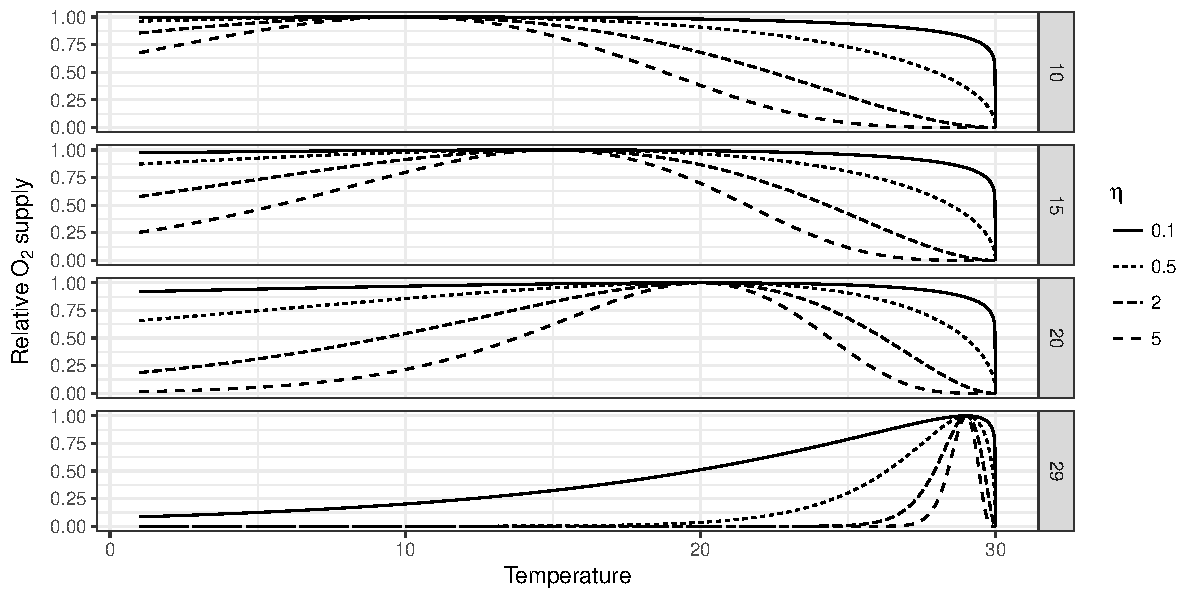
\includegraphics[width=\linewidth]{images/O2_fig-1} \caption[Maximum metabolic rate, determined by oxygen supply, as a function of temperature, for four different optimal temperatures (panels---see panel label for optimal temperature in degrees celsius), and increasing values of $\eta$]{Maximum metabolic rate, determined by oxygen supply, as a function of temperature, for four different optimal temperatures (panels---see panel label for optimal temperature in degrees celsius), and increasing values of $\eta$.}\label{fig:O2_fig}
\end{figure}




\section{Maturation-reaction norm}

\begin{figure}

{\centering \includegraphics[width=\maxwidth]{images/MRN-1} 

}

\caption[Proportion of energy allocated to reproduction, as a function of age (a) and size (b)]{Proportion of energy allocated to reproduction, as a function of age (a) and size (b). With a flat maturation-reaction norm, maturation is independent of age, and only size-dependent.}\label{fig:MRN}
\end{figure}




\end{document}
